\documentclass[border=4pt]{standalone}
\usepackage{amsmath,amssymb,amsfonts}
\usepackage{xcolor,colortbl,array,booktabs,multirow}
\usepackage{tikz}
\usepackage{pgfplots}
\pgfplotsset{compat=1.16}
\usetikzlibrary{arrows, automata, backgrounds, calendar, chains, decorations,
    matrix, mindmap, patterns, petri, positioning, shadows, shapes.geometric,
    trees, shapes, decorations.pathreplacing, calc, tikzmark, arrows.meta,
    intersections, fit, graphs, quotes, angles, decorations.markings}
\newcommand{\st}{\text{ s.t. }}
\newcommand{\x}{\mathbf{x}}
\renewcommand{\b}{\mathbf{b}}
\renewcommand{\c}{\mathbf{c}}
\newcommand{\A}{\mathbf{A}}
\newcommand{\y}{\mathbf{y}}
\newcommand{\z}{\mathbf{z}}
\newcommand{\R}{\mathbb{R}}
\newcommand{\RR}{\mathbb{R}}
\newcommand{\Z}{\mathbb{Z}}
\newcommand{\ZZ}{\mathbb{Z}}
\newcommand{\npcomplete}{NP-complete}
\providecommand{\true}{\text{TRUE}}
\providecommand{\false}{\text{FALSE}}
\tikzset{vertex/.style={circle,fill=black!25,minimum size=20pt,inner sep=0pt},
    edge/.style={draw,thick,-},weight/.style={font=\small},
    selected vertex/.style={vertex, fill=red!24},
    selected edge/.style={draw,line width=2pt,-,red!50},
    ignored edge/.style={draw,line width=2pt,-,black!20}}
\newcommand{\vect}{\vec}
\providecommand{\ds}{\displaystyle}
\providecommand{\longvect}{\overrightarrow}
\usepackage[normalem]{ulem}
\definecolor{ocre}{RGB}{243,102,25}
\providecommand{\leftB}{\left[}
\providecommand{\rightB}{\right]}
\tikzset{directed/.style={postaction={decorate,decoration={markings,mark=at position .65 with {\arrow{>}}}}},
    directed1/.style={postaction={decorate,decoration={markings,mark=at position .65 with {\arrow{>}}}}}}
\begin{document}
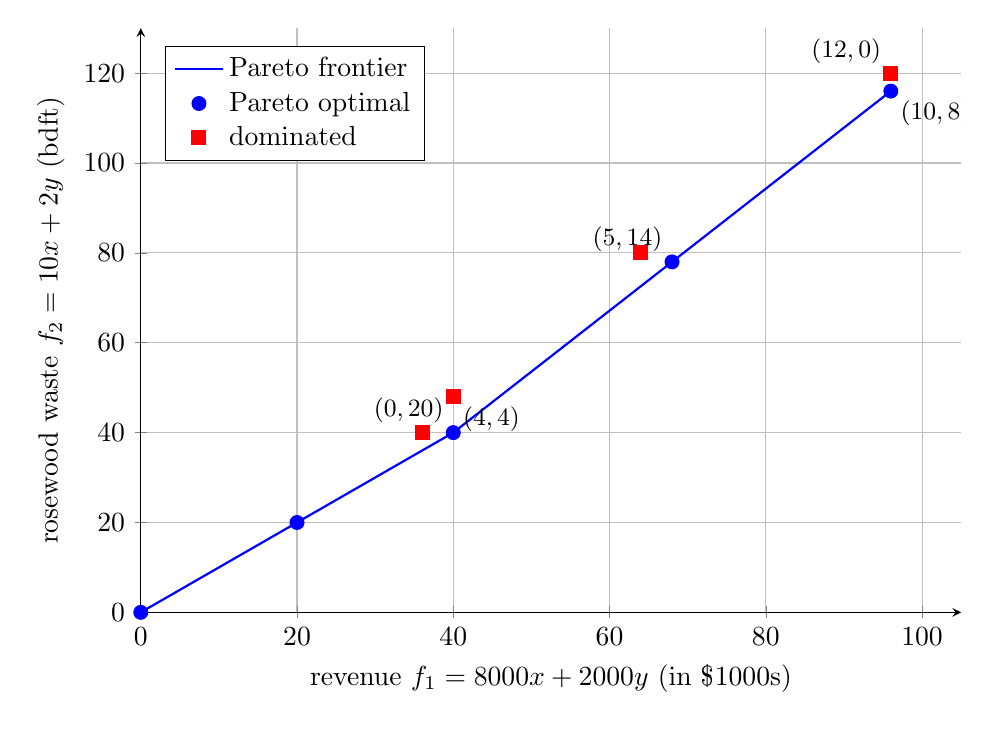
\begin{tikzpicture}
  \begin{axis}[
    xlabel={revenue $f_1 = 8000x + 2000y$ (in \$1000s)},
    ylabel={rosewood waste $f_2 = 10x + 2y$ (bdft)},
    axis lines=left,
    xmin=0, xmax=105,
    ymin=0, ymax=130,
    xtick={0,20,40,60,80,100},
    ytick={0,20,40,60,80,100,120},
    width=12cm,
    height=9cm,
    grid=both,
    enlargelimits=false,
    legend pos=north west,
    legend cell align=left,
  ]

  % Pareto frontier in objective space:
  % image of the edge x=0 (from (0,0) to (0,20)) and the edge 12x+10y=200 (from (0,20) to (10,8))
  \addplot[thick, blue] coordinates {(0,0) (40,40) (96,116)};
  \addlegendentry{Pareto frontier}

  % Pareto-optimal production plans: (0,0), (0,10), (0,20), (5,14), (10,8)
  \addplot[only marks, mark=*, mark size=2.5pt, blue] coordinates {
    (0,0) (20,20) (40,40) (68,78) (96,116)
  };
  \addlegendentry{Pareto optimal}

  % Dominated production plans: (2,10), (4,4), (8,0), (12,0)
  \addplot[only marks, mark=square*, mark size=2.5pt, red] coordinates {
    (36,40) (40,48) (64,80) (96,120)
  };
  \addlegendentry{dominated}

  % Annotate selected plans
  \node[above left, font=\small] at (axis cs:40,40) {$(0,20)$};
  \node[above left, font=\small] at (axis cs:68,78) {$(5,14)$};
  \node[below right, font=\small] at (axis cs:96,116) {$(10,8)$};
  \node[above left, font=\small] at (axis cs:96,120) {$(12,0)$};
  \node[below right, font=\small] at (axis cs:40,48) {$(4,4)$};

  \end{axis}
\end{tikzpicture}
\end{document}
